%---------------------------------------
\section{VELOCIDAD DE AVANCE DE ONDAS DE GRAN AMPLITUD} \label{sec:velocidad_grande}
%---------------------------------------
En la sección anterior se ha calculado la velocidad de avance generada para diferentes ondas viajeras bajo la suposición de oscilaciones muy pequeñas. Sin embargo, si la longitud del flagelo es considerablemente mayor que la longitud de onda y la sección de un diferencial de flagelo varía durante el desplazamiento transversal, no es posible aceptar la suposición realizada anteriormente ($ds \approx dx$) \cite{Gray1955}, y por lo tanto el diferencial de superficie ($ds$) se define por medio de la siguiente expresión
\begin{eqnarray}
	\label{eq:ds_big}
	ds = \sqrt{ 1 +\left(\frac{dy}{dx} \right)^2 } dx .
\end{eqnarray}

Además la expresión (\ref{eq:Vx_dx}) debe ser reformulada a partir las ecuaciones  (\ref{eq:dF_ds}), (\ref{eq:dF=}) y (\ref{eq:ds_big}) obteniendo que la velocidad de avance ahora se encuentra definida por: 
\begin{eqnarray}
\label{eq:Vx_dx}
	V_x (t) = \displaystyle  \frac{ (C_N - C_L) \displaystyle     \int_{0}^{\lambda}   \frac{ \frac{dy}{dt} \frac{dy}{dx} } { \sqrt{1 + \left( \frac{dy}{dx}\right)^2 } }  dx }
	{ \displaystyle  \frac{6 \pi R \mu}{n} +
	 \displaystyle   \int_{0}^{\lambda} {
		 \frac{C_L + C_N \left( \frac{dy}{dx} \right)^2}
	 			 { \sqrt{1 + \left( \frac{dy}{dx}\right)^2 } } } dx
	}
\end{eqnarray}

%---------------------------------------
\subsection{Descripción del script de integración numérica} \label{sec:descripcion_script2}
%-------------------------------------
Como consecuencia del cambio de la expresión que determina la velocidad de avance, se hace necesario modificar la función definida anteriormente para calcular la velocidad. Siendo reescrita como se muestra a continuación:
\begin{lstlisting}[]
	%% Calculo de la velocidad de avance por integración numérica.
    % Sea A = (dy/dx)^2
    
    % Vx =  (CN - CL) / sqrt(1 + A) * dy_dt * dy_dx dx 
    %       / ( Cc/n +  (CL + CN* A)  dx/ sqrt(1 + A) )

    for i=1:length(t);

      dy_dt =@(x) -(2*pi*Vp/lambda) * (c0 + c1.*x.^alfa  + c2.*x.^2)...
                  .* cos( (2*pi/lambda) * (x - Vp*t(i)) );
      
      dy_dx1 =@(x) (2*pi/lambda) .* (c0 + c1.*x.^alfa + c2.*x.^2)...
                   .* cos( (2*pi/lambda) * (x - Vp.*t(i)) );
      
      dy_dx2 =@(x) (2*c2.*x + alfa.*c1.*x.^(alfa-1))...
                   .* sin( (2*pi/lambda) * (x - Vp.*t(i)) ); 

      A = @(x) (dy_dx1(x) + dy_dx2(x)) .* (dy_dx1(x) + dy_dx2(x));

      vx_dx_num =@(x) ( (CN - CL) ./ sqrt(1 + A(x) ) )...
                      .*  dy_dt(x) .* ( dy_dx1(x) + dy_dx2(x));
                  
      vx_dx_dem =@(x)  ( CL + CN * A(x) ) ./ sqrt( 1 + A(x) ) ;
  

      % Función de integración numérica -- quadgk
      % Numerically evaluate integral, adaptive Gauss-Kronrod quadrature.
      int_num = quadgk(vx_dx_num,0,lambda);
      int_dem = quadgk(vx_dx_dem,0,lambda);

      Vx = [ Vx int_num / ( Cc/n + int_dem )];
    end

\end{lstlisting}

%---------------------------------------
\subsection{Cálculo y análisis de velocidad de onda viajera fraccionaria} \label{sec:analisis_velocidad2}
%-------------------------------------
Finalmente, se calcula las velocidades correspondiente a la ondas viajeras descritas en las Figuras \ref{fig:VCF} y \ref{fig:OVV}, cuyas magnitudes se encuentran representadas en la Figura \ref{fig:VCFB}.
\begin{figure}[!h] %  figure placement: here, top, bottom, or page
	\vspace*{3mm}
    \centering
    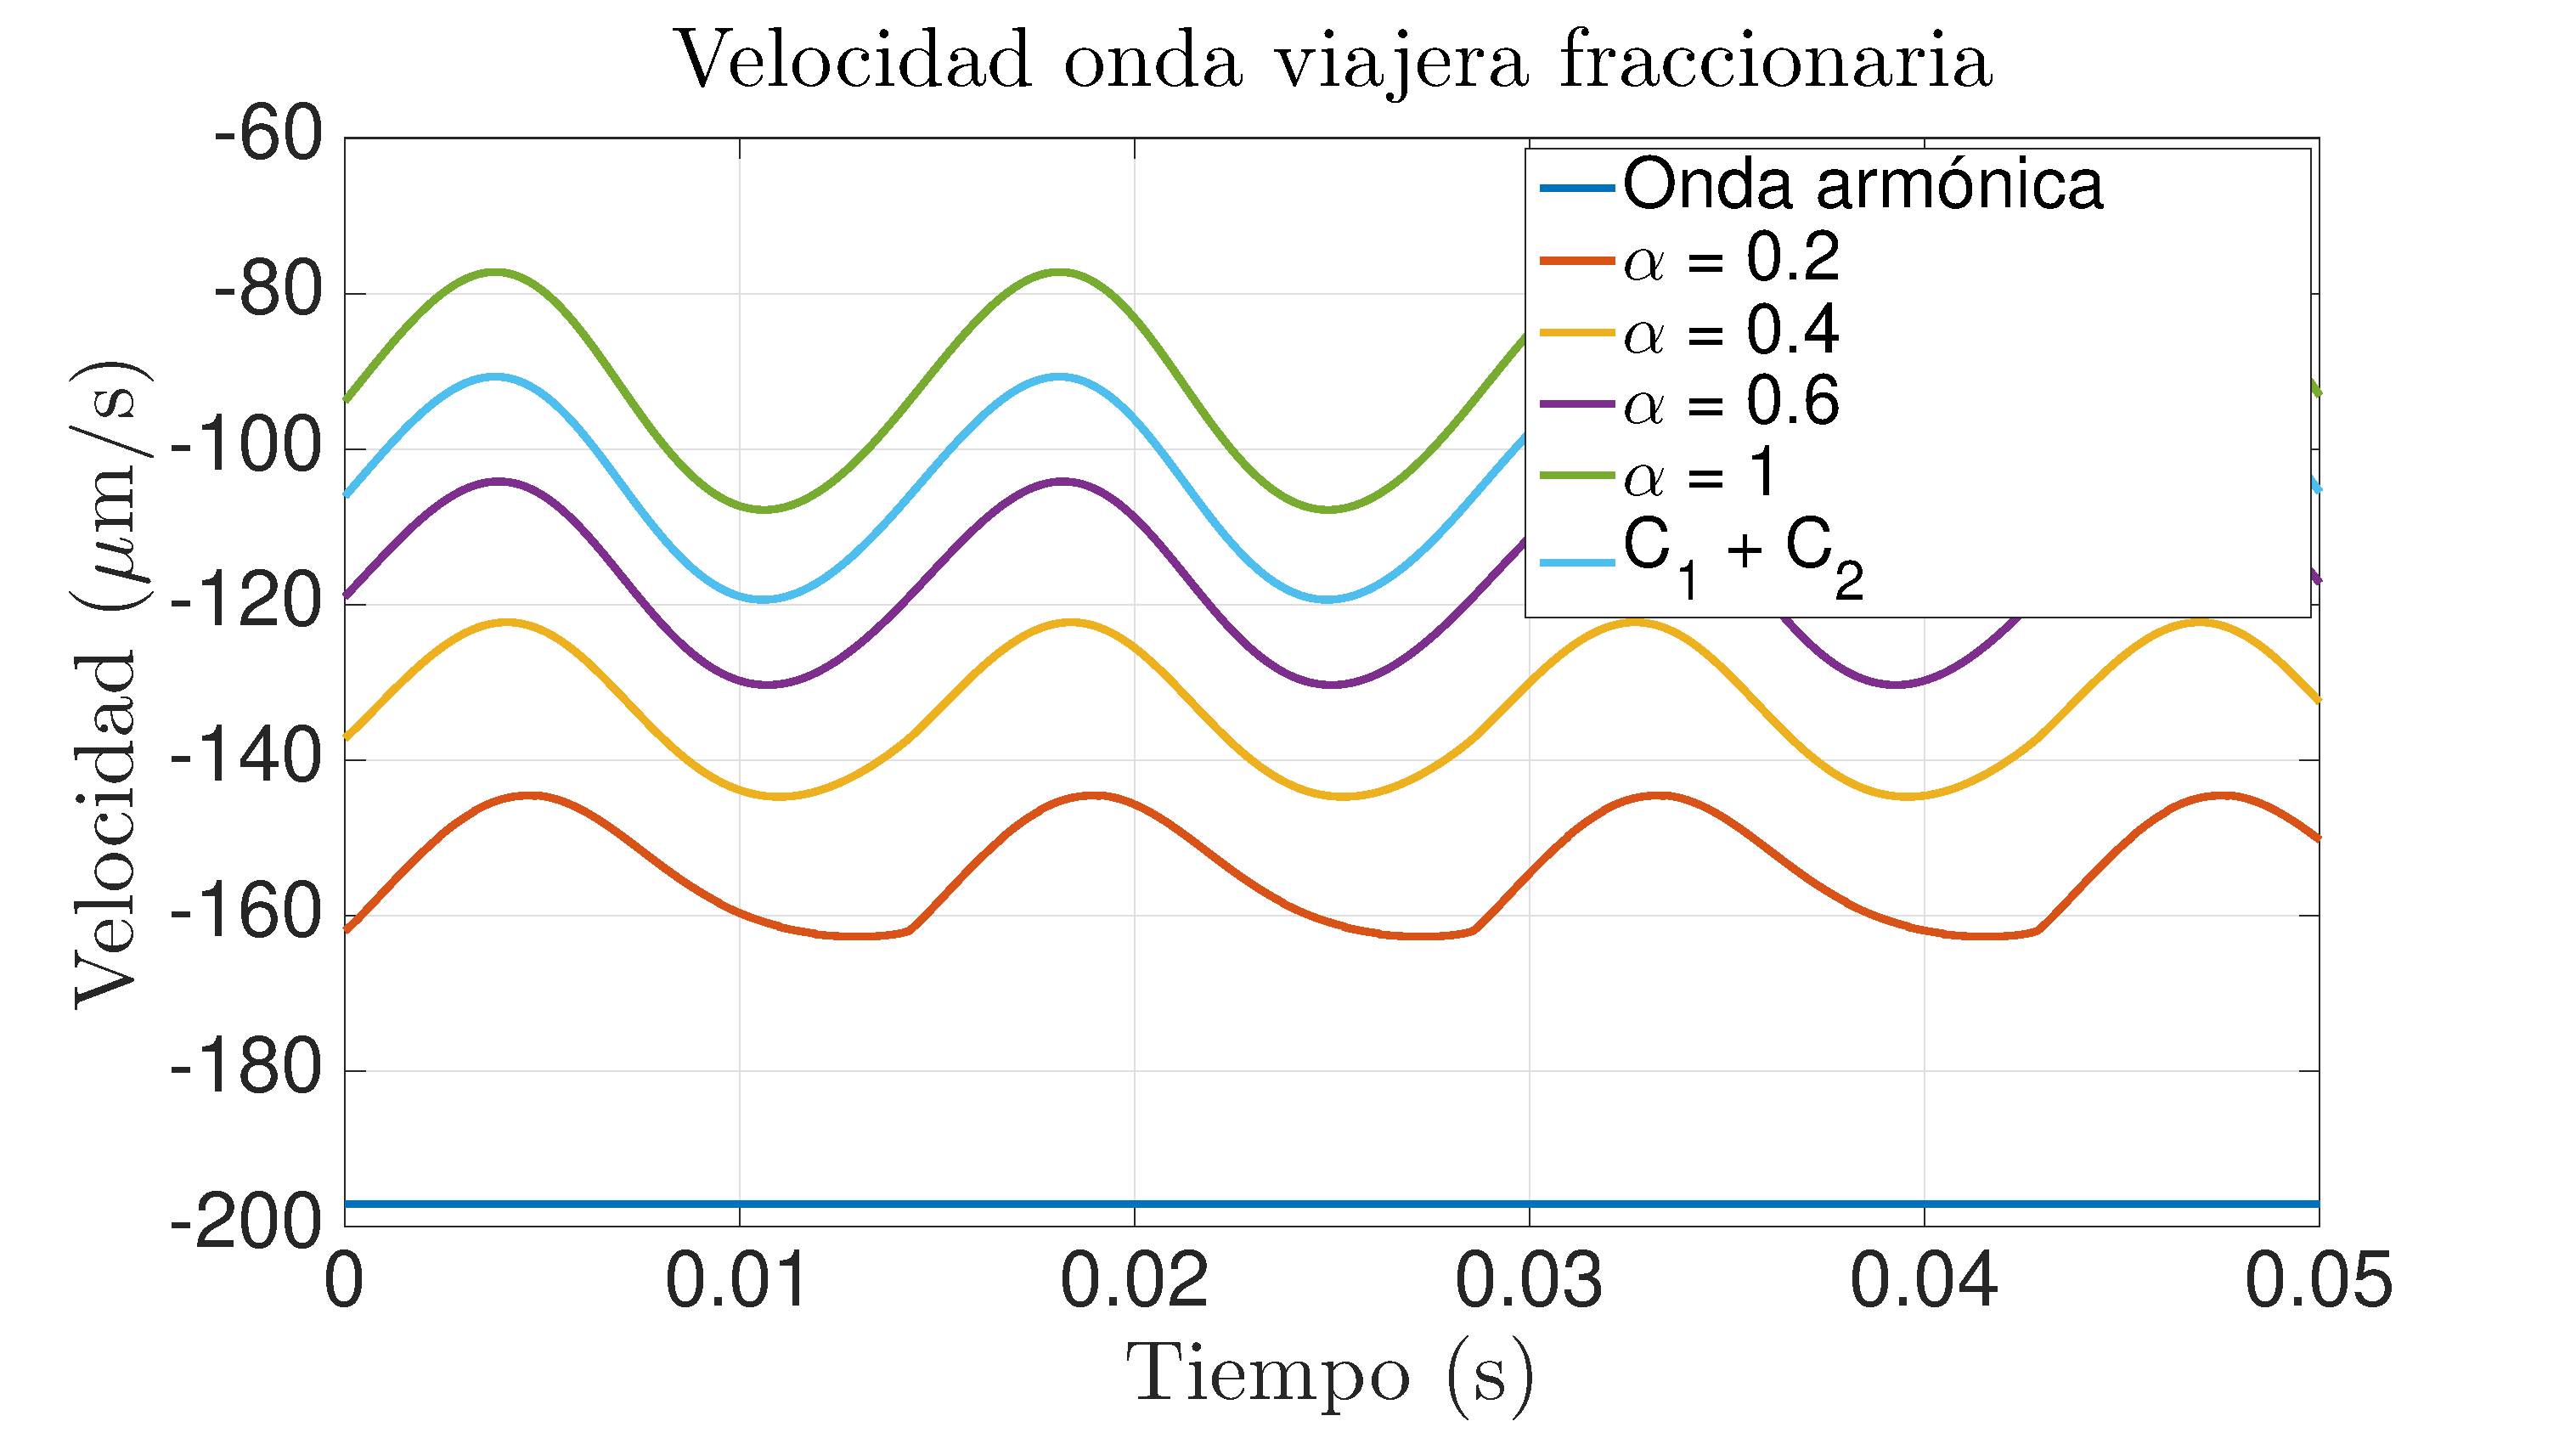
\includegraphics[width=0.85\textwidth]{Figuras/VCFB}
  	\caption{Velocidad de avance onda viajera fraccionaria de gran señal.}
  	\label{fig:VCFB}
\end{figure}

Nuevamente los resultados demuestra que la nueva expresión de onda viajera descrita proporciona una mayor velocidad de avance, aunque en esta ocasión se obtiene magnitudes menores, como consecuencia de emplear una ecuación más precisa sin el empleo de aproximaciones que simplifiquen el cálculo. Logrando un 82.23\% para un $\alpha$ = 0.2, 47.21\% y 53.81\% para el coeficiente de amplitud lineal y modulación, respectivamente.\\

También cabe destacar que la pérdida del carácter sinusoidal de la velocidad conforme disminuye el valor del parámetro $\alpha$, tal y como se muestra en la siguiente Figura \ref{fig:VCFB2}. Esto es debido a que la forma de onda cada vez alcanza una forma mas cercana a la onda armónica.
\begin{figure}[!h] %  figure placement: here, top, bottom, or page
	\vspace*{3mm}
    \centering
    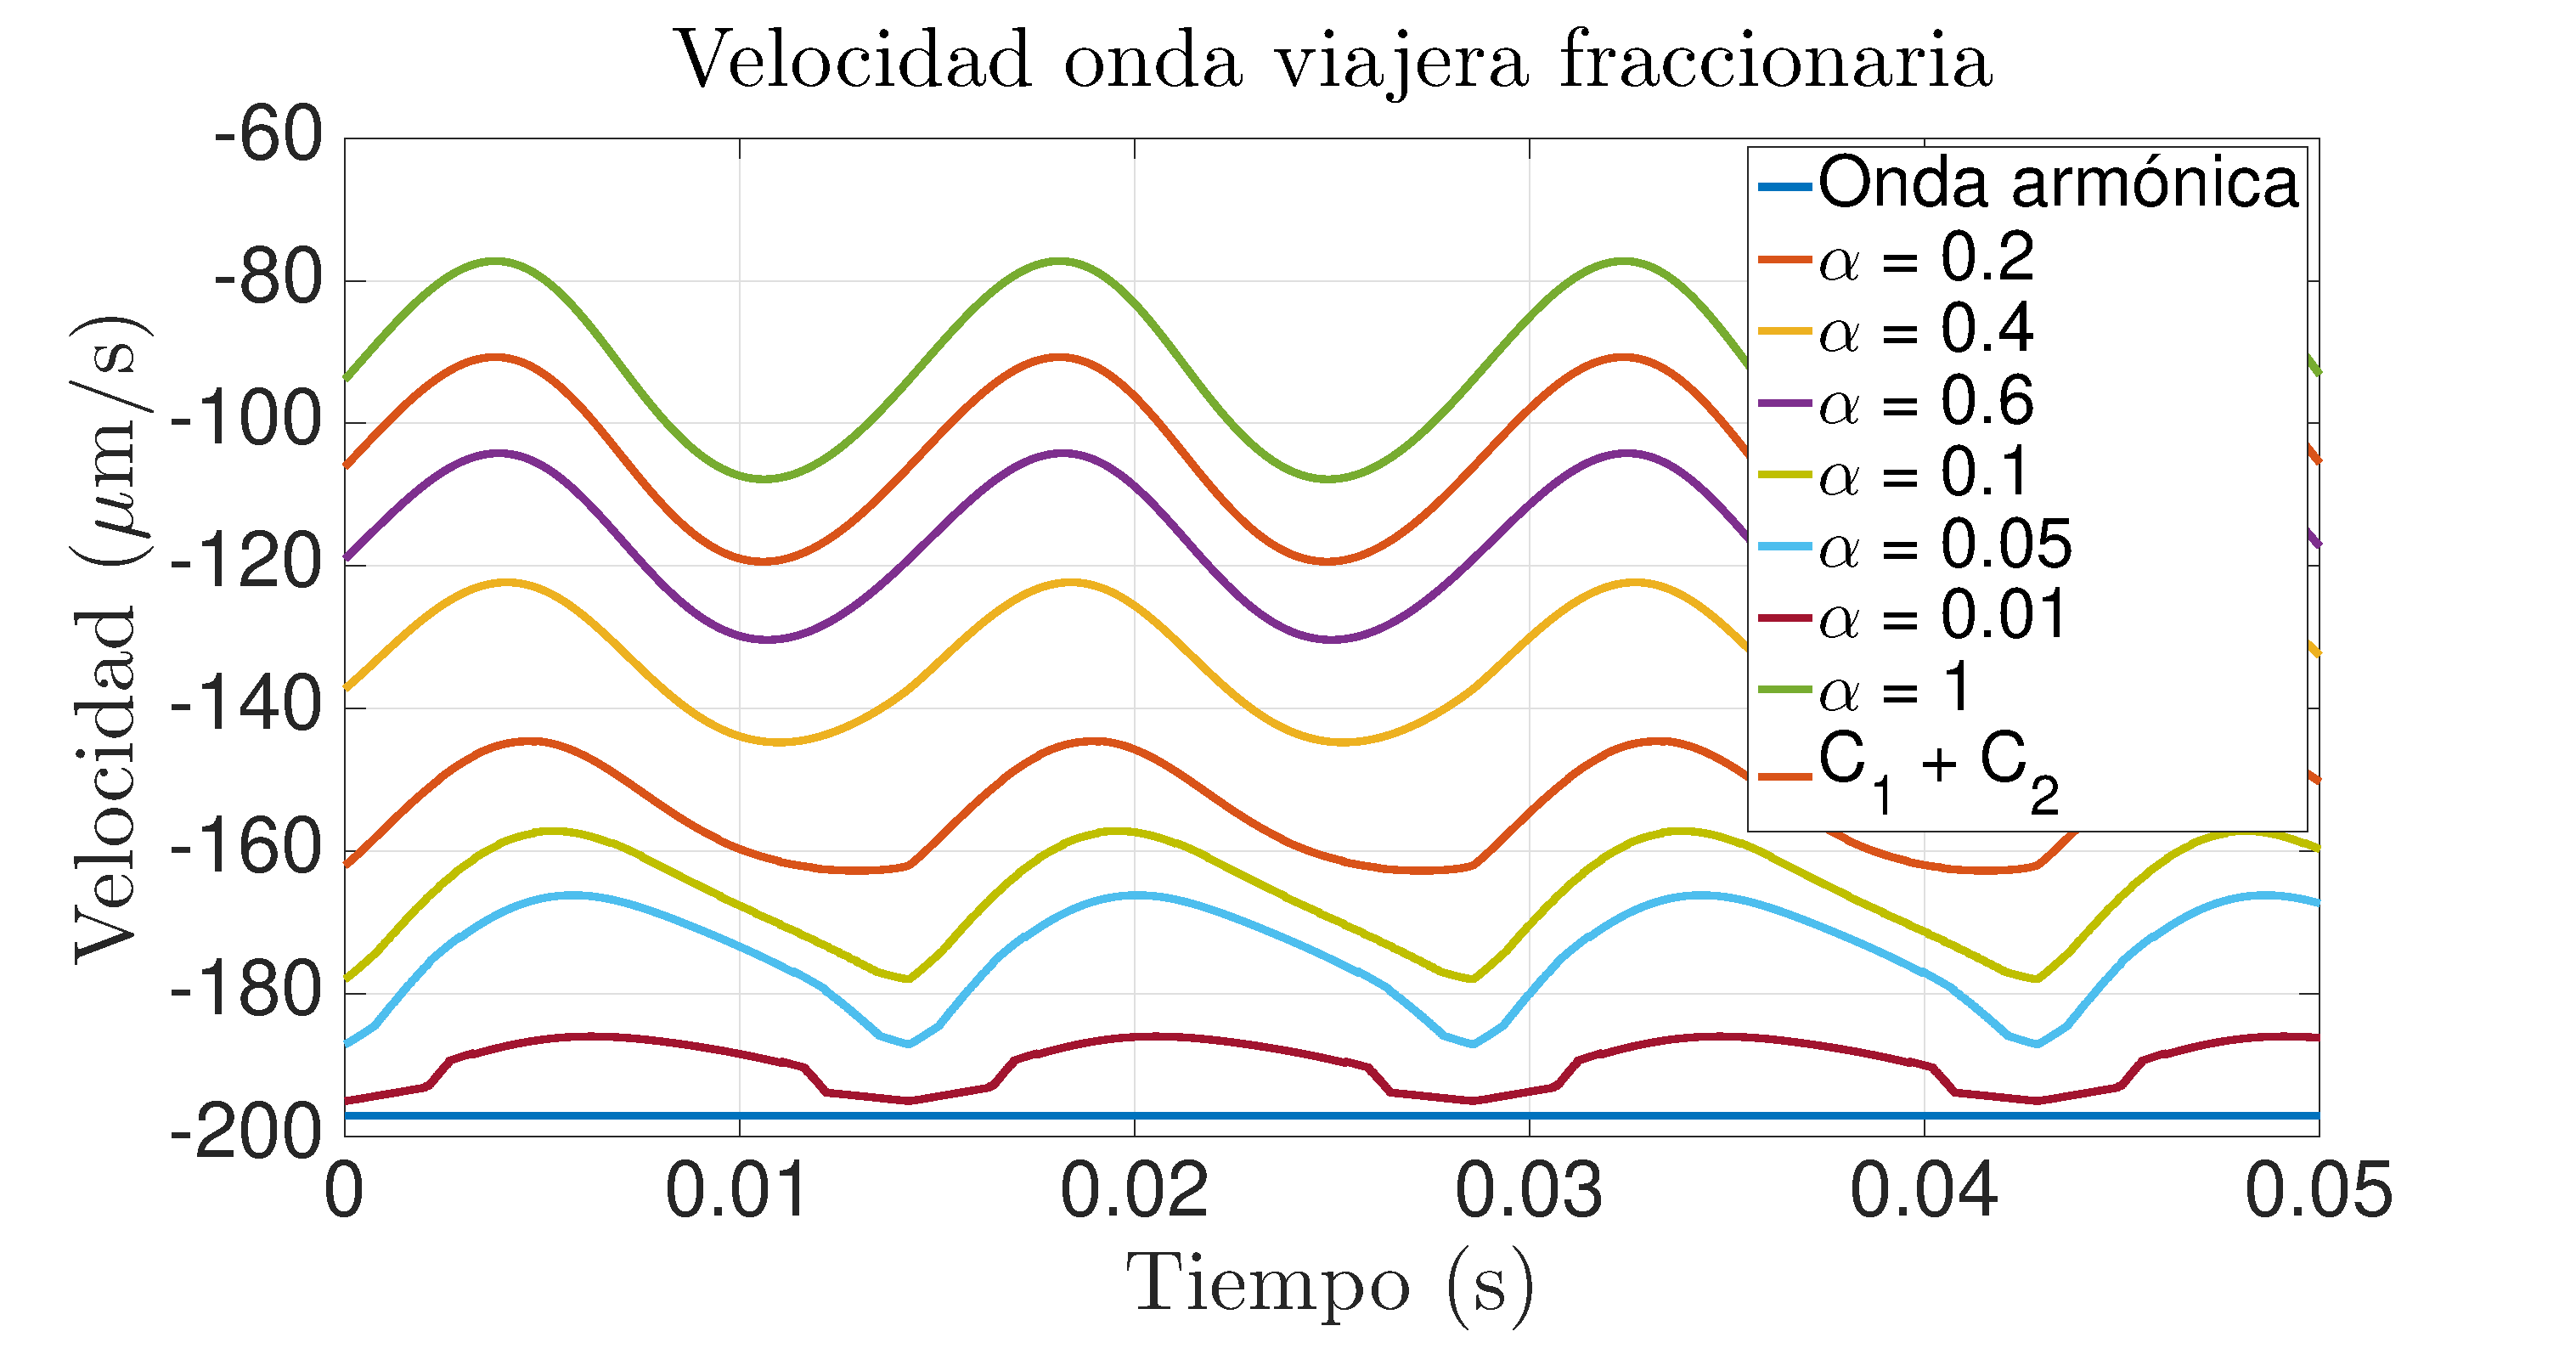
\includegraphics[width=0.85\textwidth]{Figuras/VCFB2}
  	\caption{Velocidad de avance onda viajera fraccionaria para valores bajos de $\alpha$.}
  	\label{fig:VCFB2}
\end{figure}
característica que no es tan evidente en el análisis anterior, ya que son necesario valores muy cercanos a cero para notar dicha característica.



